\newpage
\section{Durchführung und Aufbau}
\label{sec:durchfuerung}
In diesem Teil wird der Aufbau und die Durchführung des Versuchs beschrieben.
Dabei wird besonders auf die im Versuch genutzte Schaltung eingegangen.
\FloatBarrier
\subsection{Aufbau}
Zur besseren Beschreibung des Aufbaus wird dieser vereinfacht in drei Segmente geteilt: den Detektionsbereich, der Stoppuhr und dem Speicher.
Der Aufbau inklusive Schaltung kann in Abbildung \ref{fig:aufbau} gesehen werden.
\begin{figure}
    \centering
    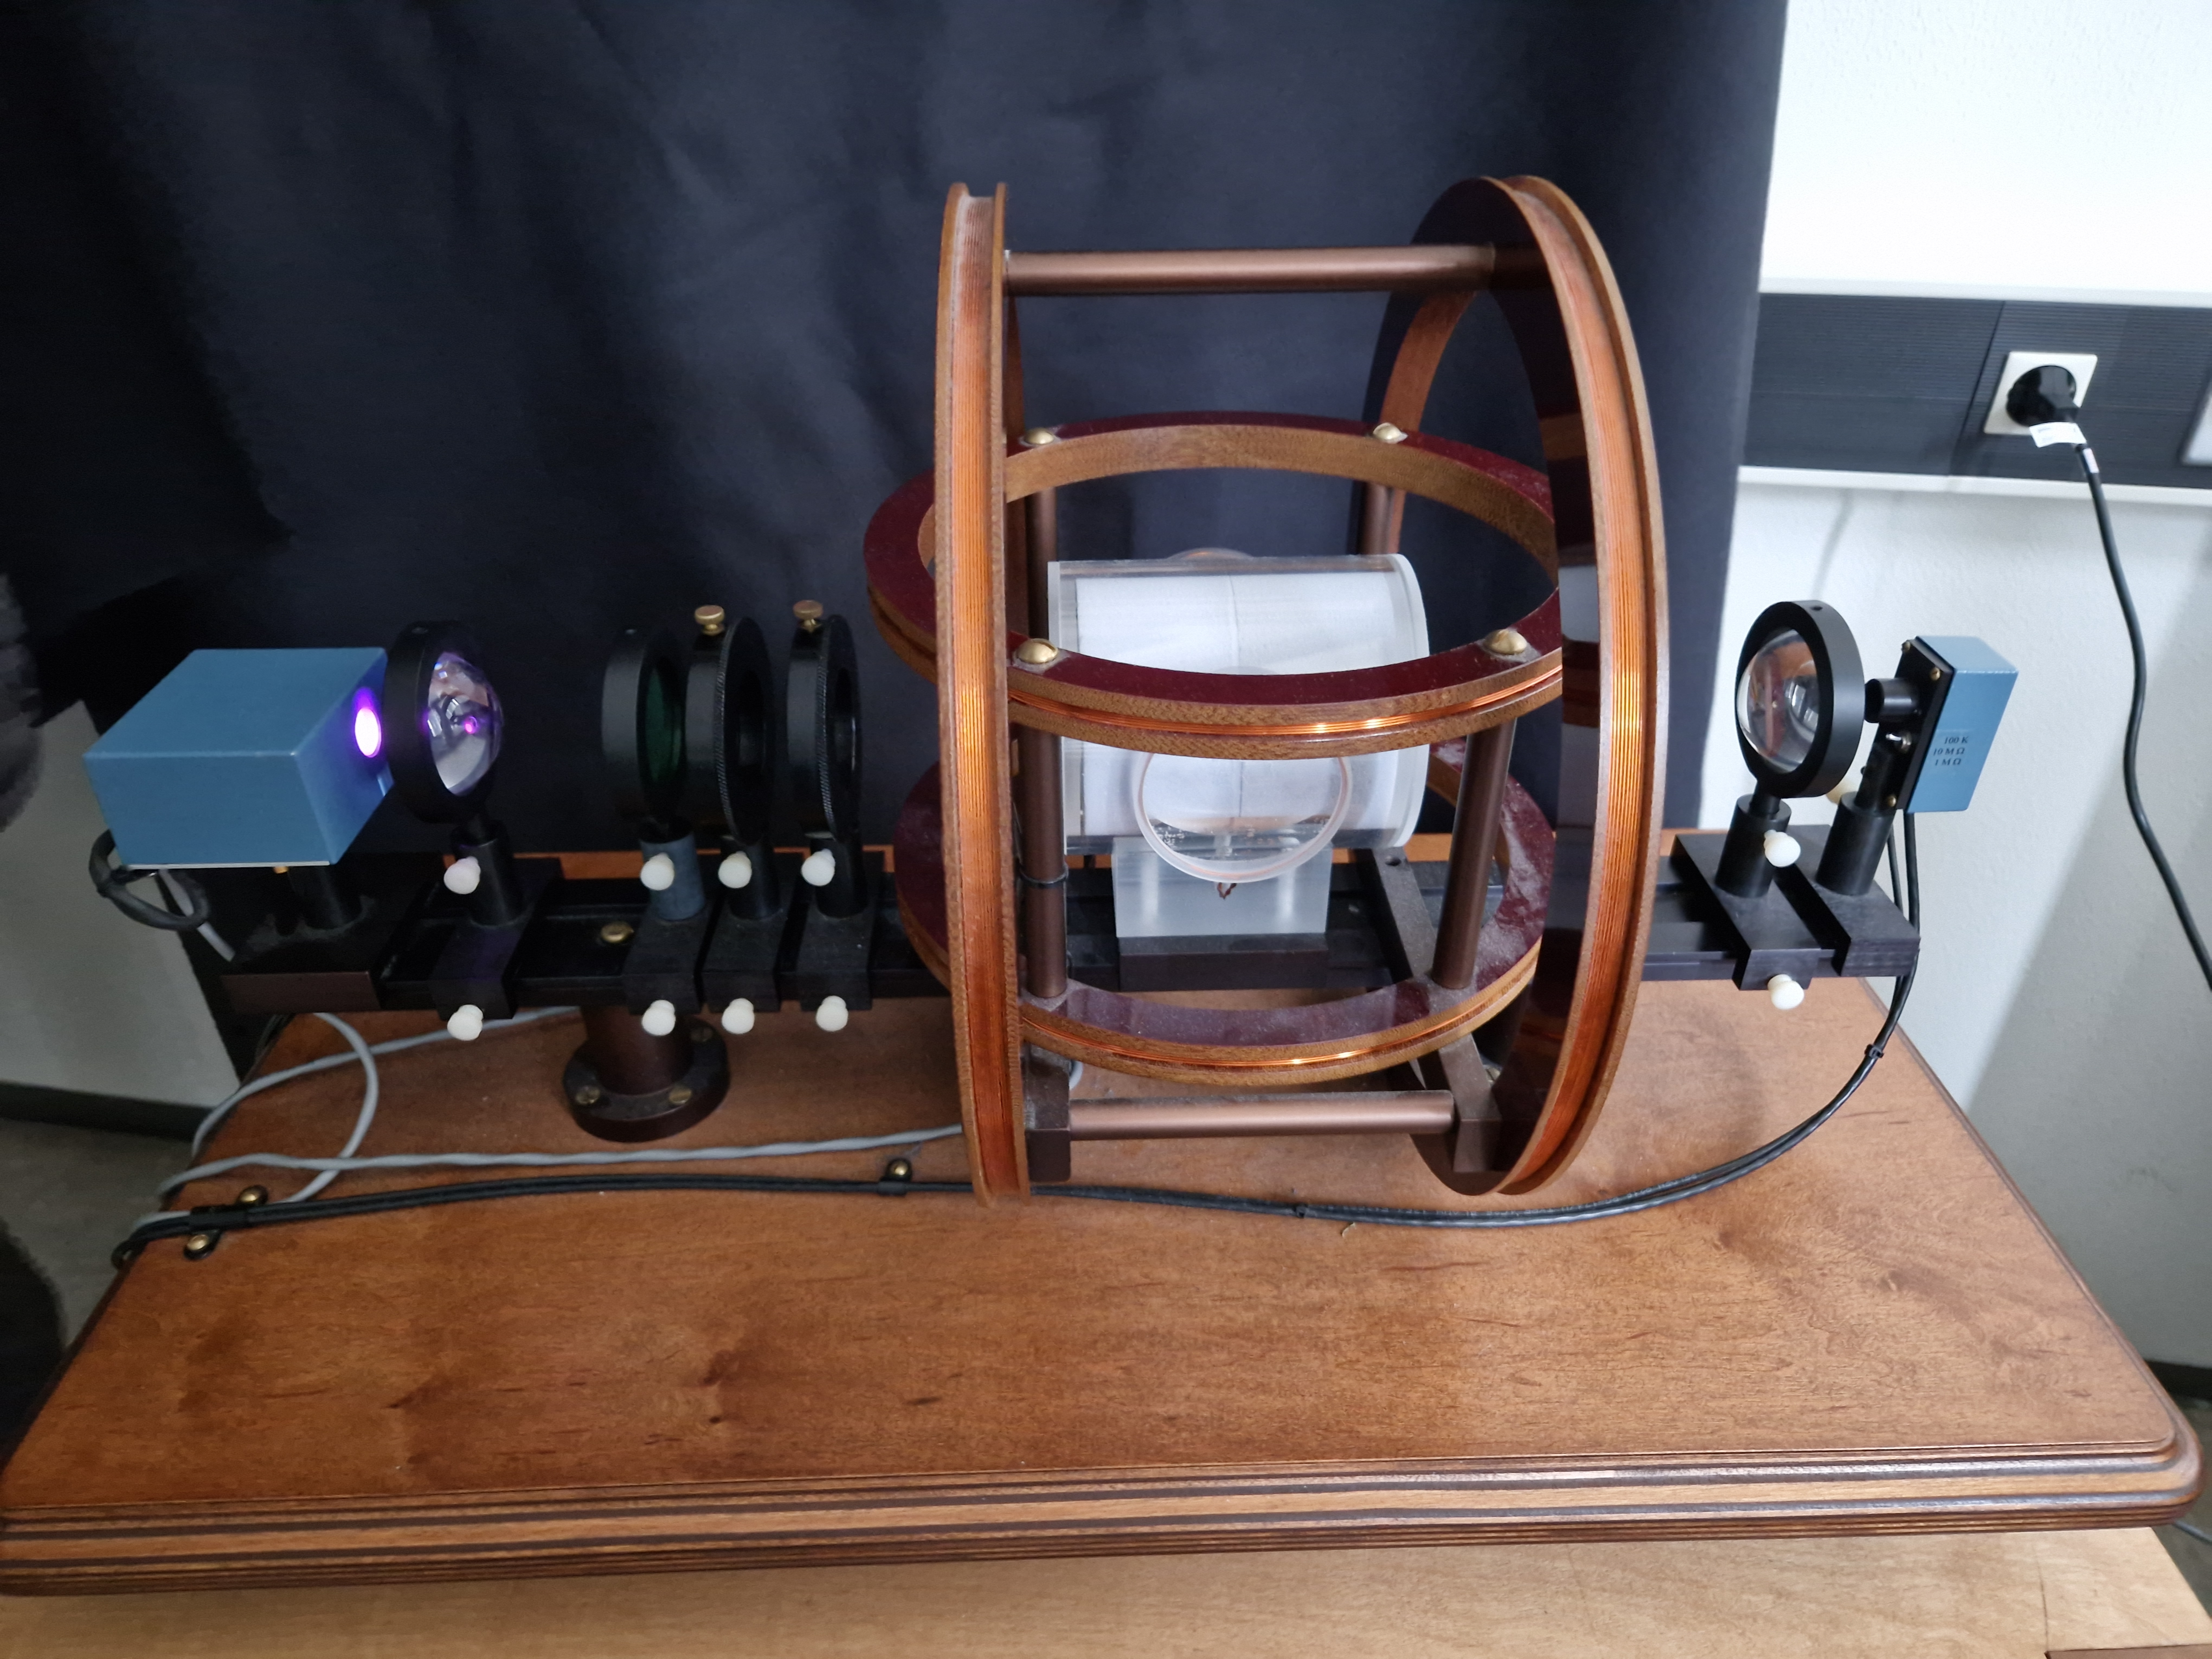
\includegraphics[width=0.65\textwidth]{data/aufbau.png}
    \caption{Eine schematische Darstellung des Aufbaus der im Versuch verwendet wird. \cite{V01}}
    \label{fig:aufbau}
\end{figure}
\FloatBarrier
\subsubsection{Detektionsbereich}
Der Detektionsbereich ist der erste der drei Teile des Aufbaus.
Er besteht aus einem Szintillatortank mit einem Volumen von ungefähr $V = \SI{50}{\litre}$.
Durch Eintreten eines Myons wir das Szintillatormaterial ionisiert, wodurch Photonen emittiert werden.
Dieser Lichtblitz kann mithilfe von zwei Photomultipliern (PMT) detektierten werden.
An den PMT liegt dabei eine Hochspannung an.
Beim Eintreten der Photonen in einen der PMT wird dabei eine Elektronenkaskade ausgelöst.
Diese erzeugt letztendlich ein Spannungssignal, welches in die Schaltung gegeben wird.\\
Aber nicht nur beim Eintritt eines geladenen Teilchens wird ein Lichtblitz erzeugt sondern auch beim Zerfall.
Im Fall des Myons liegt es daran, dass es in ein Elektron sowie zwei Neutrinos zerfällt.
Die Neutrinos haben im Vergleich zu den Myonen eine nur geringe Masse.
Die Masse des Myons ist im Vergleich zum Elektron groß.
Aufgrund dieser Massendifferenz hat das entstandene Zerfalls Elektron eine hohe kinetische Energie.
Diese kinetische Energie deponiert das Elektron in Form von Photonen im Szintillatortank.\\
Diese Photonen könne von den PMT gemessen werden.
Um möglichst wenig Fehlmessungen zu erhalten werden zwei PMTs genutzt, die beide ein Signal messen müssen damit die Stoppuhr aktiviert wird.
In diesem Kontext ist eine Fehlmessung, die Ausgabe eines Signals durch ein PMT obwohl kein Myon in das Detektorvolumen eingetreten ist.
Aus diesem Grund werden an beide PMT jeweils eine Verzögerungsleitung angeschlossen.
Diese sorgt dafür, dass die Spannungsimpulse der PMTs gleichzeitig an der Koinzidenz ankommen.
Zwischen PMT und Koinzidenz befindet sich zudem ein Diskriminator, welcher dafür sorgt, dass nur genügend große Spannungsimpulse durchgelassen werden.
Wenn zwei Spannungsimpulse gleichzeitig an der Koinzidenz ankommen gibt diese ein Signal weiter an den Stoppuhr-Bereich der Schaltung.
\subsubsection{Stoppuhr}
Die Koinzidenz gibt ihr Signal weiter an den Stoppuhr-Teil der Schaltung.
Das Koinzidenz Signal wird dabei an zwei AND-Gatter und einen Monoflop weiter gegeben.
Der Monoflop erhält das Signal allerdings erst nachdem dieses durch eine Verzögerungsleitung gelaufen ist.
An dem Monoflop wird die Suchzeit $T_\text{such}$ eingestellt, während der die Stoppuhr aktiv bleibt.\\
Solange kein Signal an der Stoppuhr angekommen ist, gibt der Monoflop an das AND Gatter 1 ein WAHR und an das AND Gatter 2 ein FALSCH Signal.
Wenn nun ein Signal in die Stoppuhr eingeht, bekommt das AND Gatter 1 zwei WAHR Signale und aktiviert damit den Time-Amplitude-Converter (TAC).
Außerdem invertiert der Monoflop, nachdem das Signal durch die Verzögerung gelaufen ist, sein Ausgangssignal.
Wenn nun ein zweites Signal durch die Koinzidenz kommt erhält AND Gatter 2 zwei WAHR Signale und stoppt so den TAC.
Der TAC wandelt dann die Zeit in der dieser aktiv war in ein Spannungssignal um.
Dabei ist dessen Amplitude größer, umso länger der TAC aktiv war.
Der TAC gibt sein Spannungssignal an das Speicher-Segment der Schaltung weiter.
Nachdem die Suchzeit $T_\text{such}$ des Monoflops um ist stellt sich dieser wieder in seine Grundeinstellung und eine neue Messung kann beginnen.
\subsubsection{Speicher}
Der TAC gibt sein Ausgangssignal an einen Multi-Channel-Analyzer (MCA) weiter.
Dieser ordnet jedem Signal einen Kanal zu.
Die Zuordnung hängt dabei von der Amplitude des Signals ab.
Umso Höher die Amplitude des Signal, umso höher ist auch die Kanalnummer.
Da die Amplitude des Signals proportional zu der gemessenen Zerfallszeit ist, muss während der Kalibration gemessen werden welcher Kanalnummer welche Zerfallszeit entspricht.\\
Zusätzlich zum MCA sind zwei Impulszähler teil des Speicher Segments der Schaltung.
Diese messen wie oft AND Gatter 1 und 2 aktiviert werden.
Daraus lässt sich später feststellen wie viele Fehlmessungen es gab.
\subsection{Durchführung}
Die Schaltung wird nach Abbildung \ref{fig:aufbau} aufgebaut.
Nach dem Verkabeln der Schaltung muss diese kalibriert werden.
Dabei wird bei der Detektoreinheit angefangen.\\
Zunächst müssen die Diskriminatoren kalibriert werden.
Dafür wird das Ausgangssignal eines Diskriminators in ein Oszilloskop gegeben.
Nun wird die Pulsbreite des Ausgangssignal so angepasst, dass diese eine ungefähre Halbwertsbreite von $\SI{15}{\nano\second}$ hat.
Dieselbe Einstellung wird ebenfalls für den anderen Diskriminator durchgeführt.\\\\
Als nächstes werden die beiden Verzögerungsleitungen zwischen PMT und Diskriminator so angepasst, dass die Koinzidenz ein Signal ausgibt, wenn beide PMT einen Lichtblitz messen.
Dafür wird an die Koinzidenz ein Impulszähler angeschlossen.
Nun wird die Verzögerung einer Verzögerungsleitung variiert und für ein Messintervall von $\Delta t = \SI{10}{\second}$, gemessen wie viele Impulse die Koinzidenz ausgibt.
Es werden für beide Verzögerungsleitungen die Impulse bei Verzögerungen von $(0-15)\,\si{\nano\second}$ gemessen.
Nachdem die Messreihe abgeschlossen ist, wird eine Verzögerung gewählt, bei welcher ungefähr 20 Impulse pro Sekunde durch die Koinzidenz gelassen werden.\\\\
An dem Monoflops wird eine Suchzeit von $T_\text{such} = \SI{14}{\micro\second}$ eingestellt.
Der Messbereich des TAC wird dementsprechend angepasst.
Wenn dieser nicht angepasst wird, werden die ausgegebenen Amplituden zu klein oder zu groß sein.
Dies führt dazu, dass die Empfindlichkeit der Messung eingeschränkt wird.\\\\
Um die Kanalnummern einer Messzeit zuzuordnen, wird der MCA kalibriert.
Dafür wird ein Doppelimpulsgenerator anstelle der Koinzidenz gesetzt, der zwei Impulse generiert, dessen zeitlicher Abstand in einem Intervall von $(0.3-9.9)\,\si{\micro\second}$ einstellbar ist.
Wenn nun eine Zeit an dem Doppelimpulsgenerator eingestellt wird, so wird der TAC Spannungsimpulse gleicher Amplitude an den MCA geben.
Dadurch füllt dieser nur einen Kanal, welcher zu der Zeit gehört, die am Doppelimpulsgenerator eingestellt wird.
Um möglichst genau die Kanalnummer zu einem Zeitintervall zuordnen zu können, werden die Kanalnummern für mehrere Zeitintervalle am Doppelimpulsgenerator bestimmt.
Es werden 20 Zeitintervalle von $(0.3-9.9)\,\si{\micro\second}$ in $0,5\,\si{\micro\second}$-Schritten gemessen.\\\\
Nach der vollständigen Kalibration wird der Doppelimpulsgenerator aus der Schaltung entfernt.
Die Koinzidenz wird wieder in die Schaltung integriert und die eigentliche Messung wird gestartet.
Nach ungefähr 3 Tagen wird die Messung gestoppt.